
\subsection{The transformer encoder layer}\label{sec:transformer encoder}
The previously described elements are now aggregated into a transformer encoder layer.
To improve the performance of the transformer, multiple of these layers can be stacked, and each of these encoder layers contain a self-attention sublayer as well as a feedforward sublayer. 

Once the multi-head attention weights have been computed, these weights are then fed into a dropout layer that has a residual connection consisting of the initial query.
Given some rate value, this layer randomly sets the input units to 0 using that rate as the dropout frequency.
In other words, some values from the input are dropped, which helps prevent overfitting during training.

Following the dropout layer, the weights are normalized in a normalization layer. 
This gives us the final attention weights, which are then passed to the feedforward layer.

The feedfoward layer is the dense layer, as described in section \ref{sec:multi-head attention}.
It should be noted that the two dense layers per encoder layer consist of 1-dimensional convoluted neural networks with a kernel size and stride of 1.
The output of these two layers are then fed into another dropout layer, which also has a residual connection consisting of the initial query. 

Finally, the values are normalized, which gives us the final transformer encoder output values.
The resulting architecture can be seen in figure \ref{fig:encoder transformer}.
As this figure demonstrates, the architecture is different from the original transformer architecture shown in figure \ref{fig:original transformer}.
Our transformer architecture is inspired by the architecture presented by \citet{schmitz_stock_2020}, which includes many of the original architectural elements from \textit{Attention Is All You Need}\cite{AttentionIsAllYouNeed}.
Because we are not working with natural language processing, there is no need for a decoder layer, since we do not to output any decoded data. 

\begin{figure}[h]
\centering
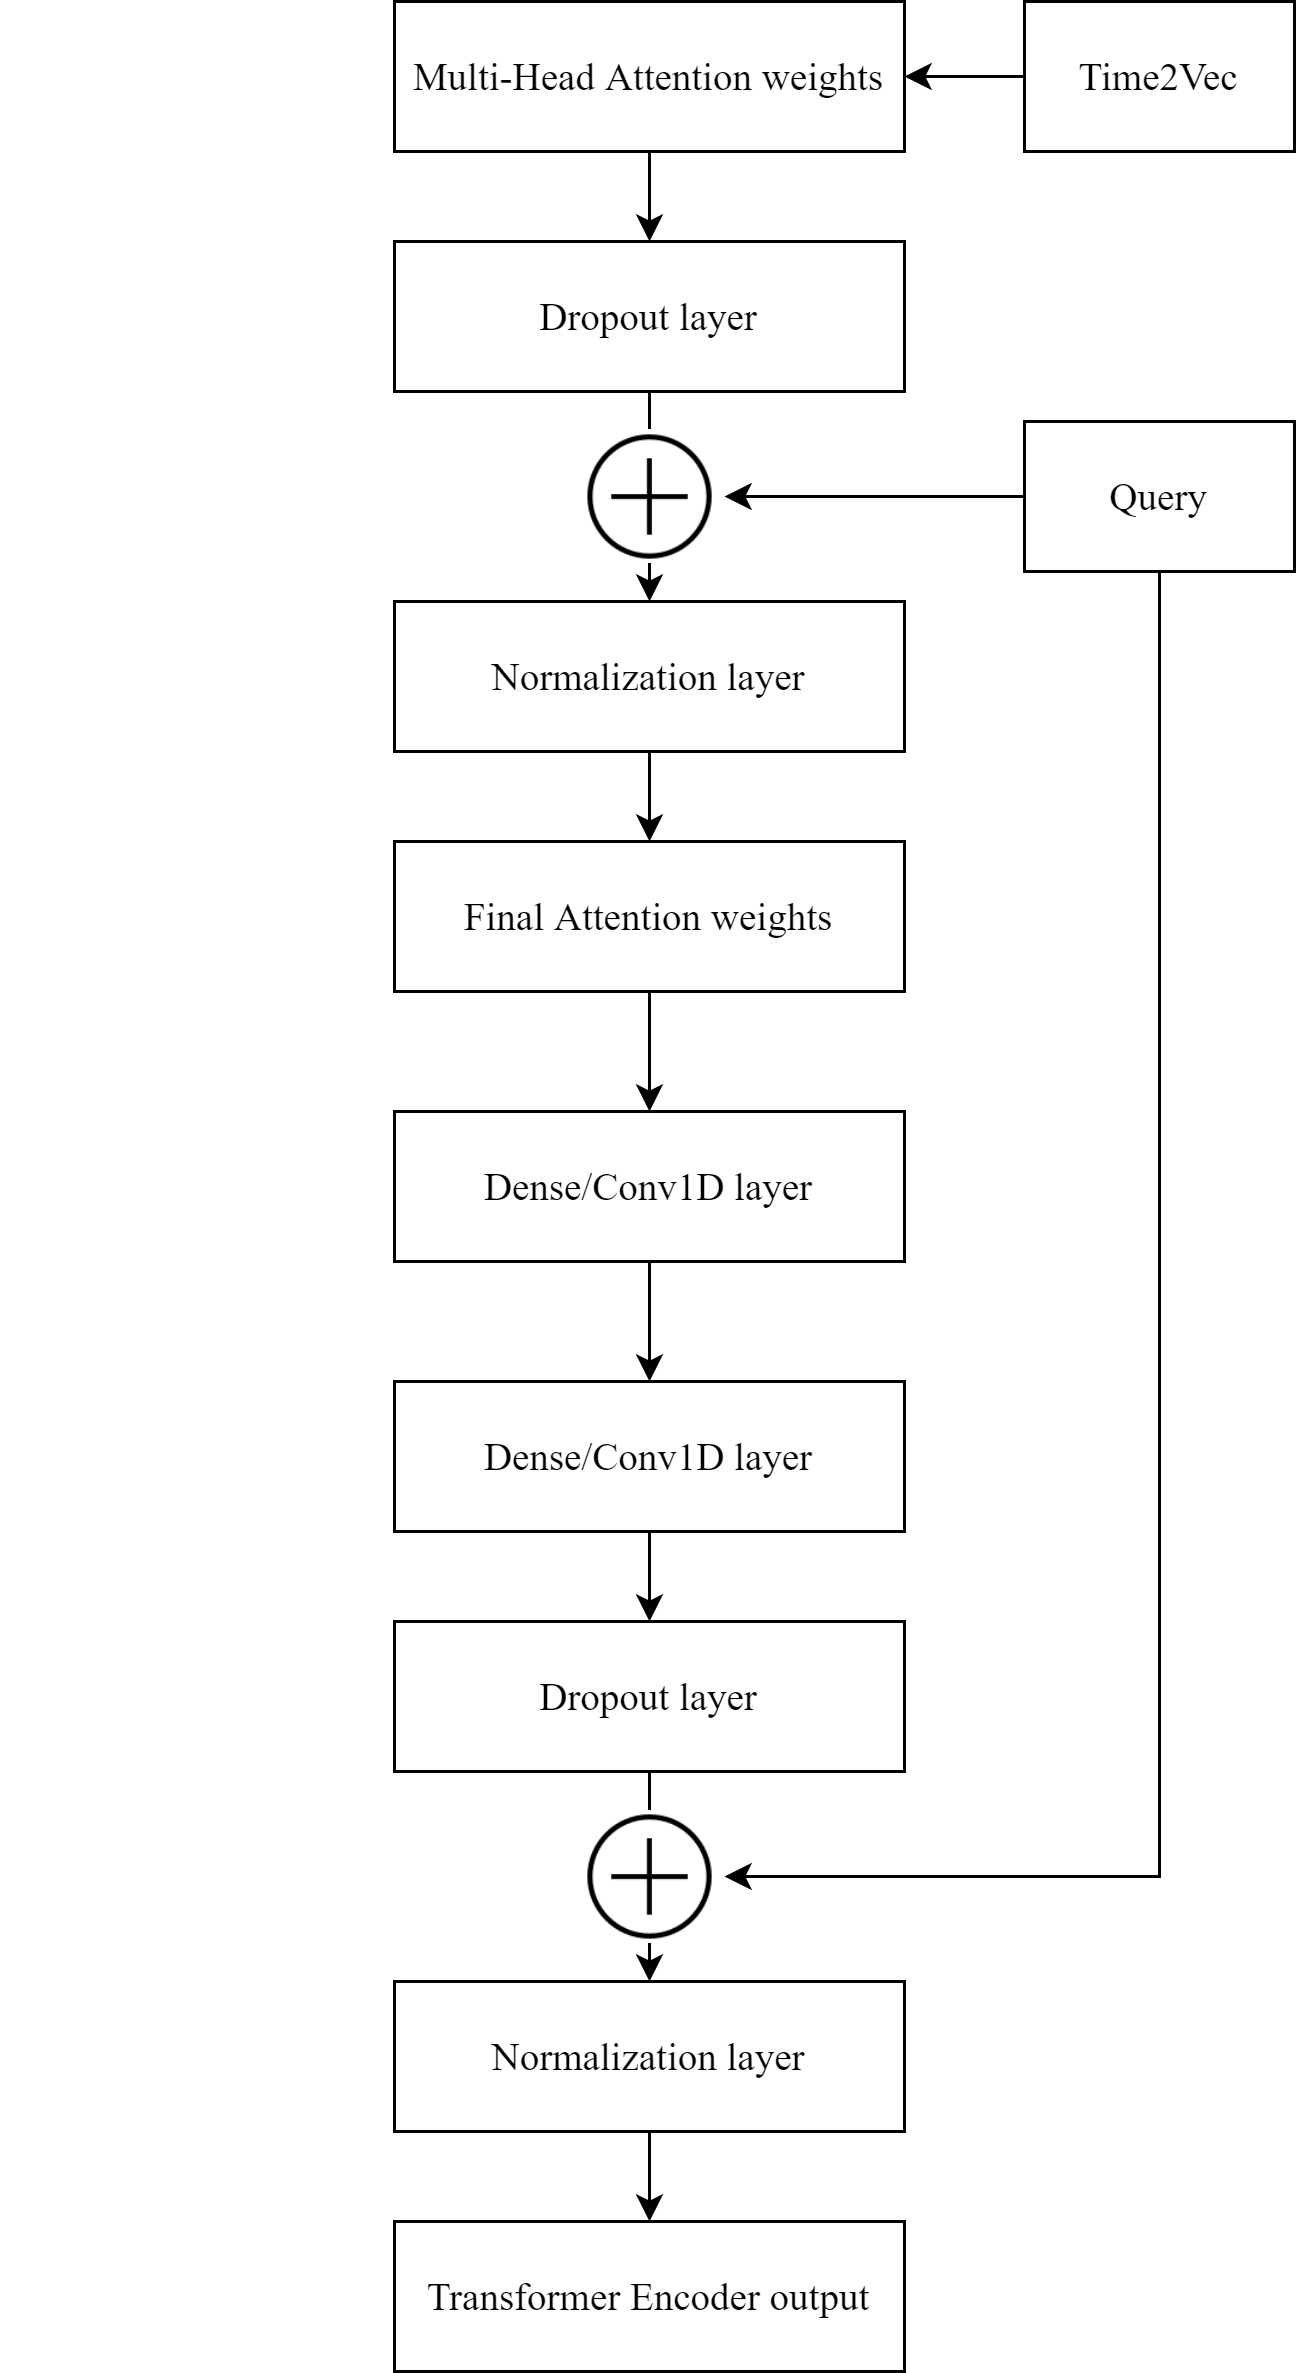
\includegraphics[width=0.375\textwidth]{Encoder transformer}
\caption{The transformer encoder layer.}
\label{fig:encoder transformer}
\end{figure}